\documentclass[a4paper, amsfonts, amssymb, amsmath, reprint, showkeys, nofootinbib, twoside]{revtex4-1}
\usepackage[spanish]{babel}
\usepackage[utf8]{inputenc}
\usepackage{float}
\usepackage[colorinlistoftodos, color=green!40, prependcaption]{todonotes}
\usepackage{amsthm}
\usepackage{mathtools}
\usepackage{physics}
\usepackage{xcolor}
\usepackage{graphicx}
\usepackage[left=23mm,right=13mm,top=35mm,columnsep=15pt]{geometry} 
\usepackage{adjustbox}
\usepackage{placeins}
\usepackage[T1]{fontenc}
\usepackage{lipsum}
\usepackage{csquotes}
\usepackage[normalem]{ulem}
\useunder{\uline}{\ul}{}
\usepackage[pdftex, pdftitle={Article}, pdfauthor={Author}]{hyperref} % For hyperlinks in the PDF
%\setlength{\marginparwidth}{2.5cm}
\bibliographystyle{apsrev4-1}

\begin{document}

%El título del experimento realizado es importante.
\title{Espectros de átomos y espectografía}


\author{David Santiago Pachon Ballen}
\email[Correo institucional: ]{d.pachonb@uniandes.edu.co}

%Si necesitan poner un segundo autor, deben eliminar los porcentajes (%) iniciales.
  
\author{Sergio Montoya Ramírez}
\email{s.montoyar2@uniandes.edu.co}

\affiliation{Universidad de los Andes, Bogotá, Colombia.}

\date{\today} % Si lo dejan vacío no les saldrá fecha. La fecha que se muestra es del día en que se compila.

\begin{abstract}

En este se describen brevemente los objetivos y los resultados del trabajo, por lo tanto se debe dar información completa pero corta del contenido del trabajo. Se debe indicar qué fue lo que se hizo, cómo se hizo y cuáles fueron los resultados obtenidos.

\end{abstract}

\maketitle
\section{Objetivos}
\begin{enumerate}
    \item Medir las longitudes de onda emitidas por un átomo de hidrógeno y comprobar que se ajustan a la fórmula de Balmer
    \item Determinar la constante de Rydberg
    \item Medir algunas lineas espectrales de otros elementos
    \item Grabar con una cámara varios espectros de lineas de emisión
    \item Observar 4 lineas de hidrógeno
    \item Usar el espectro del hidrógeno para calibrar la escala horizontal de las imágenes
    \item Con la escala calibrada medir las longitudes de onda de otros espectros
    \item Medir la estructura fina de la linea amarilla del mercurio
\end{enumerate}
\section{Introducción}
Uno de los métodos mas potentes para la identificación de elementos es la espectroscopia en donde un elemento que es excitado con energía después de un tiempo en el que la perturbación haya acabado emite esta energía en forma de radiación electromagnética. Además, cada sistema lo hace diferente, en particular el hidrógeno produce un espectro como el que aparece en la figura \ref{fig:Ehidrogeno}
\begin{figure}[H]
    \centering
    \includegraphics[scale=0.6]{Ehidrogeno_Teorico.jpeg}
    \caption{Espectro de absorción del hidrógeno, tomado de las diapositivas del profesor}
    \label{fig:Ehidrogeno}
\end{figure}
Por otro lado la formula teorica que describe la longitud de onda correspondiente a cada línea de la serie espectral fue dada por J. Balmer y es la siguiente
$$\lambda = \frac{3647n^2}{n^2-4}A$$
donde n es el número entero que identifica cada línea de la serie. Por otro lado J. Rydberg propuso que esta misma formula se escribiera de la siguiente manera
$$\frac{1}{\lambda} = R_H\left[ \frac{1}{2^2}-\frac{1}{n^2}\right]$$
donde $R_H$ es una constante experimental y que se denomina constante de Rydberg. \cite{Unal_Moderna}
\section{Montaje experimental}
\begin{figure}[H]
  \centering
  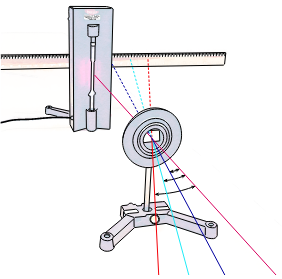
\includegraphics[scale=0.5]{Graficas/procedimiento.png}
  \caption{Figura de representación del Montaje experimental. En esta, aparecen una regla, un tubo espectral, la fuente, una rejilla de digracción y un soporte.}
  \label{fig:procedimiento}
\end{figure}
Una vez acomodado el montaje experimental como indica en la figura \ref{fig:procedimiento} debemos acomodar la camara. En particular, para este experimento utilizamos un celular Redmi Note 7. El celular, fue acomodado detras de la rejilla de difracción por medio de un estante. 

Luego de esto, se instalo un tubo de hidrógeno en posición vertical a la fuente que posteriormente haria pasar electrones por el gas y por tanto haria que ilumine.  Una vez hecho esto, acomodamos la regla de manera que el 1 se encuentre alineado con el tuvo de hidrógeno y en la camara se observe la posición de los haces de luz como se puede observar en la foto \ref{fig:calibrar}.

Luego de hacer esto, repetimos el procedimiento para otro gas. En esta caso, utilizamos el neon con el cual obtuvimos resultados similares.

\section{Resultados y análisis}

Una vez tomamos la figura \ref{fig:calibrar}
\begin{figure}[H]
    \centering
    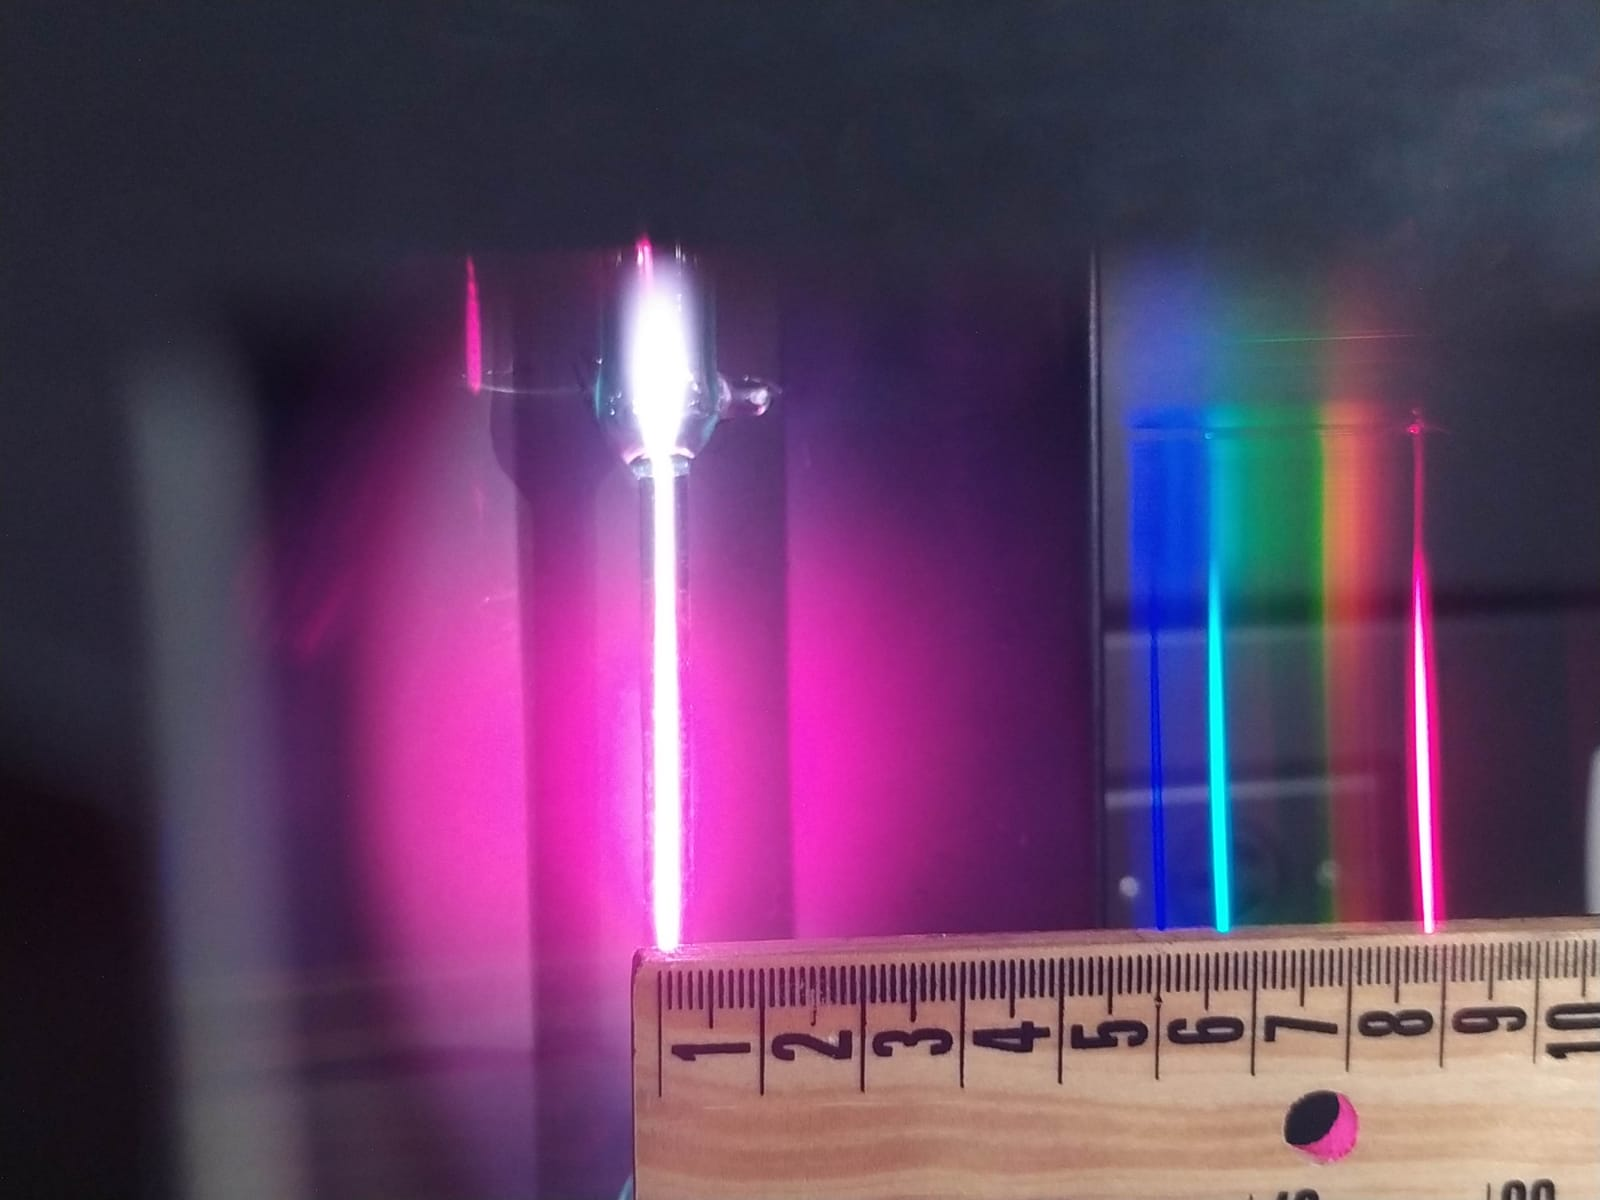
\includegraphics[scale=0.1]{Hidrogeno_Zoom.jpeg}
    \caption{Imagen tomada en el laboratorio en donde se observa el espectro de emisión del hidrogeno. Esta fue realizada siguiendo las indicaciones del montaje experimental. En la imagen se observa a la derecha el tubo de hidrógeno que emite la luz. A la izquierda, se ven las ondas de emisión del hidrógeno. En particular, podemos observar las de longitud de onda 410, 434, 656}
    \label{fig:calibrar}
\end{figure}
 la pasamos por el programa Fiji/ImageJ el cual es un programa de análisis de imagen. En esta caso lo primero que hacemos es retirar los colores como aparece en la figura \ref{fig:CalibrarBN}. 
 \begin{figure}[H]
     \centering
     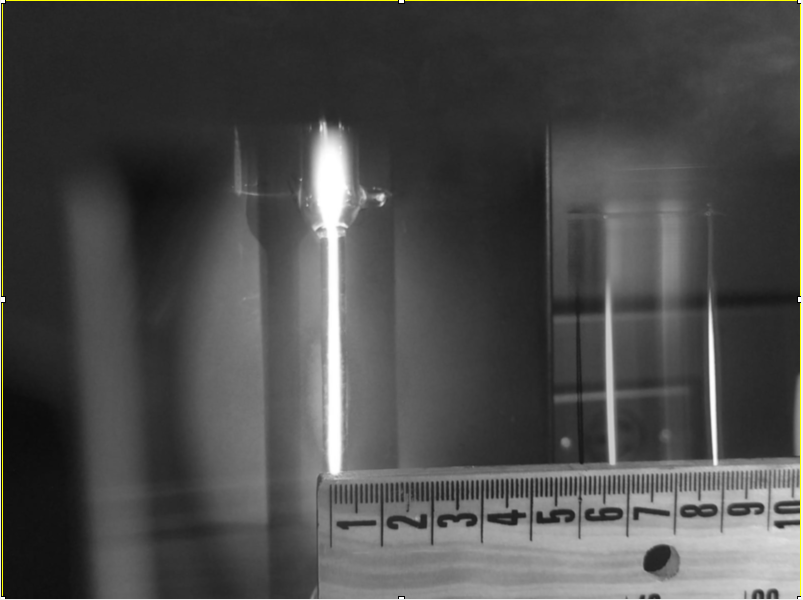
\includegraphics[scale=0.3]{Graficas/Hidrogeno_BN.png}
     \caption{Primer paso del análisis de la imagen \ref{fig:calibrar}. Este es solamente el retiro de los colores para quedar con una imagen en escala de grises. Note que una de las lineas resulta converger en negro en vez de converger a blanco como se esperaba.}
     \label{fig:CalibrarBN}
 \end{figure}
 Una vez hecho esto, utilizamos otra herramienta del mismo software con la cual nos permite analisar la escala de grises que tiene en función de una distancia. Un ejemplo de esta grafica se muestra en la imagen \ref{fig:Hidrogeno}.
\begin{figure}[H]
    \centering
    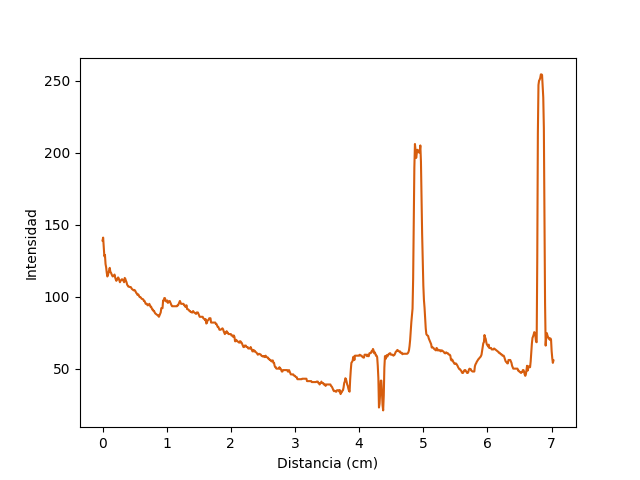
\includegraphics[scale=0.5]{Graficas/Hidrogeno.png}
    \caption{Grafica distancia vs intensidad luminica, esta se realizo con el software Fiji ImageJ con la cual se análiso la equivalencia de cada punto con su escala de grises.}
    \label{fig:Hidrogeno}
\end{figure}
Una vez tenemos esta información, gracias a que tenemos la teoria podemos hallar la relación que hay entre la distancia y la longitud de onda. Para esto aprovechamos la grafica \ref{fig:Hidrogeno} ya que de esta sabemos cuales son las longitudes de onda que estamos buscando. La relación entre estas lineas y la distancia esta en la tabla \ref{table:calibrar}.
\begin{table}[h]
    \centering
    \caption{Tabla de longitud de Onda vs distancia, con la distancia registrada en el programa y los conocimientos teoricos se adquieren estos datos para calibrar la función de longitud de onda en relación a la distancia.}
    \label{table:calibrar}
    \begin{tabular}{|c|c|}
        \hline
        \hline
        Longitud de Onda (nm) & Distancia (cm)\\
        \hline
        410 & 4,2\\
        434 & 4,9\\
        486 & 6,8\\
        \hline
        \hline
    \end{tabular}
\end{table}

Una vez tenemos esto lo ponemos en una grafica y hacemos una regresión lineal que nos permite saber su pendiente y su punto de corte, lo cual nos da una función polinomial que es la que representa la longitud de onda vs la distancia recorrida. Esta imagen es la figura 
\begin{figure}[H]
    \centering
    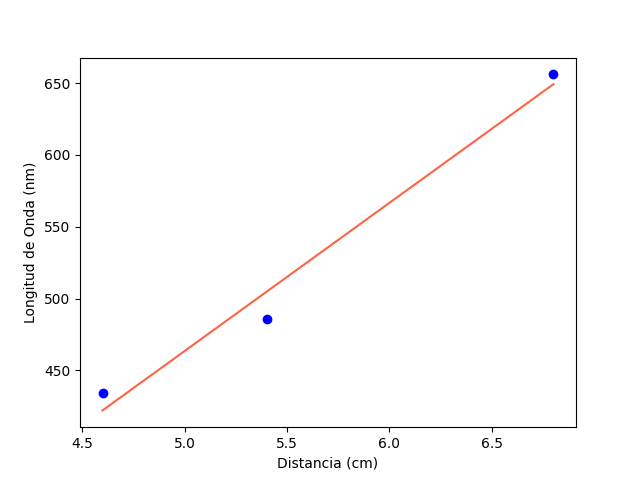
\includegraphics[scale=0.5]{Graficas/Flambda.png}
    \caption{Grafica de distancia vs longitud de onda para las longitudes de onda teoricas del hidrogeno. Ademas, en esta aparece la función que relaciona la distancia con la longitud de onda calibrada con los datos del hidrogeno. En concreto los datos de esta función son m = 34.83 y b = 248.2}
    \label{fig:Flambda}
\end{figure}
Una vez tenemos esto, realizamos la primera parte del análisis. Es decir, hasta encontrar la grafica de intensidad vs distancia. Esta grafica es la \ref{fig:Helio}.
\begin{figure}[H]
  \centering
  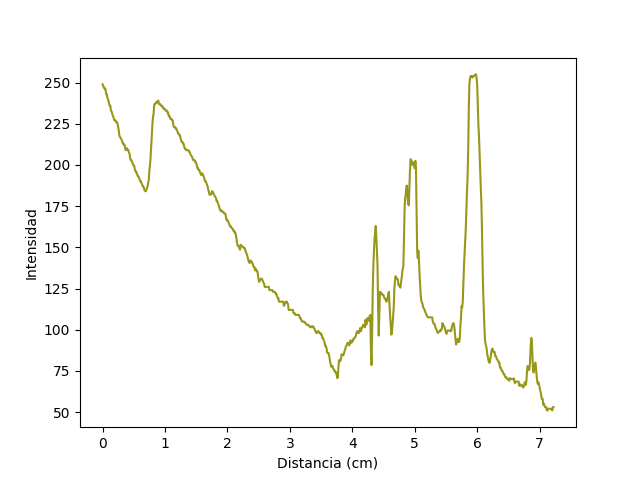
\includegraphics[scale=0.5]{Graficas/Helio.png}
  \caption{Grafica distancia vs intensidad luminica, esta se realizo con el software Fiji ImageJ con la cual se análiso la equivalencia de cada punto en la escala de grises.}
  \label{fig:Helio}
\end{figure}
Una vez que tenemos esta, identificamos los picos presentes y pasamos su posición por nuestra función de longitud de onda vs distancia. Los resultados se encuentran en la tabla \ref{table:Flambda}
\begin{table}[h]
    \centering
    \caption{Tabla de longitudes de Onda en función de un n para el helio. Estos datos fueron hayados gracias a la función polinomial encontrada previamente, representada en la figura \ref{fig:Flambda}.}
    \label{table:Flambda}
    \begin{tabular}{|c|c|}
        \hline
        \hline
        Frecuencia & n \\
        \hline
        405 & 1 \\
        422 & 2\\
        457 & 3\\
        485 & 4\\
        \hline
        \hline
    \end{tabular}
\end{table}
Por ultimo, se grafican estos datos de una manera especial pues la pendiente de esa grafica nos da la constante de Rydberg. Esta es una grafica de $\frac{1}{4}-\frac{1}{n^2}$ vs $ \frac{1}{\lambda}$ de esta manera la pendiente nos deja R.
\begin{figure}[H]
    \centering
    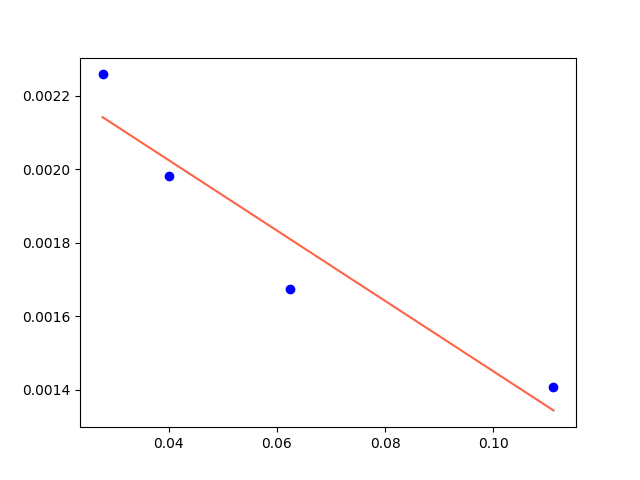
\includegraphics[scale=0.5]{Graficas/grafica_mr.png}
    \caption{Gracfica de $\frac{1}{4}-\frac{1}{n^2}$ vs $\frac{1}{\lambda}$ con el objetivo de encontrar la constante de Rydberg que es en este caso la pendiente de la grafica.}
    \label{fig:mr}
\end{figure}
\section{Conclusiones}

Se logro medir las longitudes de onda emitidas por un átomo de hidrógeno y calibrar una relación entre la distancia y la longitud de onda que ocasiona una línea espectral en este punto. Sin embargo, la precisión de la misma no resulto suficientemente alta pues las longitudes de onda encontradas para el helio no resultaron exactos. No se logro determinar la constante de Rydberg con suficiente exactitud dado que el resultado dado que el valor experimental que conseguimos fue 27.5 lo cual difiera ampliamente con el resultado esperado.Se consiguio medir algunas lineas espectrales de otros elementos, en particular, se logro mostar las lineas espectrales del Helio como se ve en la figura \ref{fig:Helio}.Conseguimos grabar con una cámara varios espectros de lineas de emisión esto queda registrado y demostrado en la figura \ref{fig:calibrar}.Se consigui observar lineas del hidrógeno y esto se muestra en varios de las figuras puestas asi como en la tabla \ref{table:Flambda}.Se logro calibrar la escala horizontal de las imágenes usando las lineas de hidrogeno. Esto, queda registrado en la explicación de la grafica \ref{fig:Flambda}. Se lograron medir las longitudes de onda de otros espectros utilizando la función calibrada con las lineas de H. Sin embargo, esta no fue suficientemente preciso debido a la incapacidad de encontrar los limites exactos. Por lo tanto, la practica de laboratorio cumplio algunos de los objetivos que se plantearon en un inicio.

\bibliographystyle{abbrv}
\bibliography{Referencias}

\end{document}
